\appendix
\chapter{Higher-Order-Transformations}\label{appendix:hots}
The following figures illustrate the in this Master's Thesis created \ac{HOT}s,
which transform given Henshin edit rules into profiled ones.
 \begin{figure}[h!]
\begin{center}
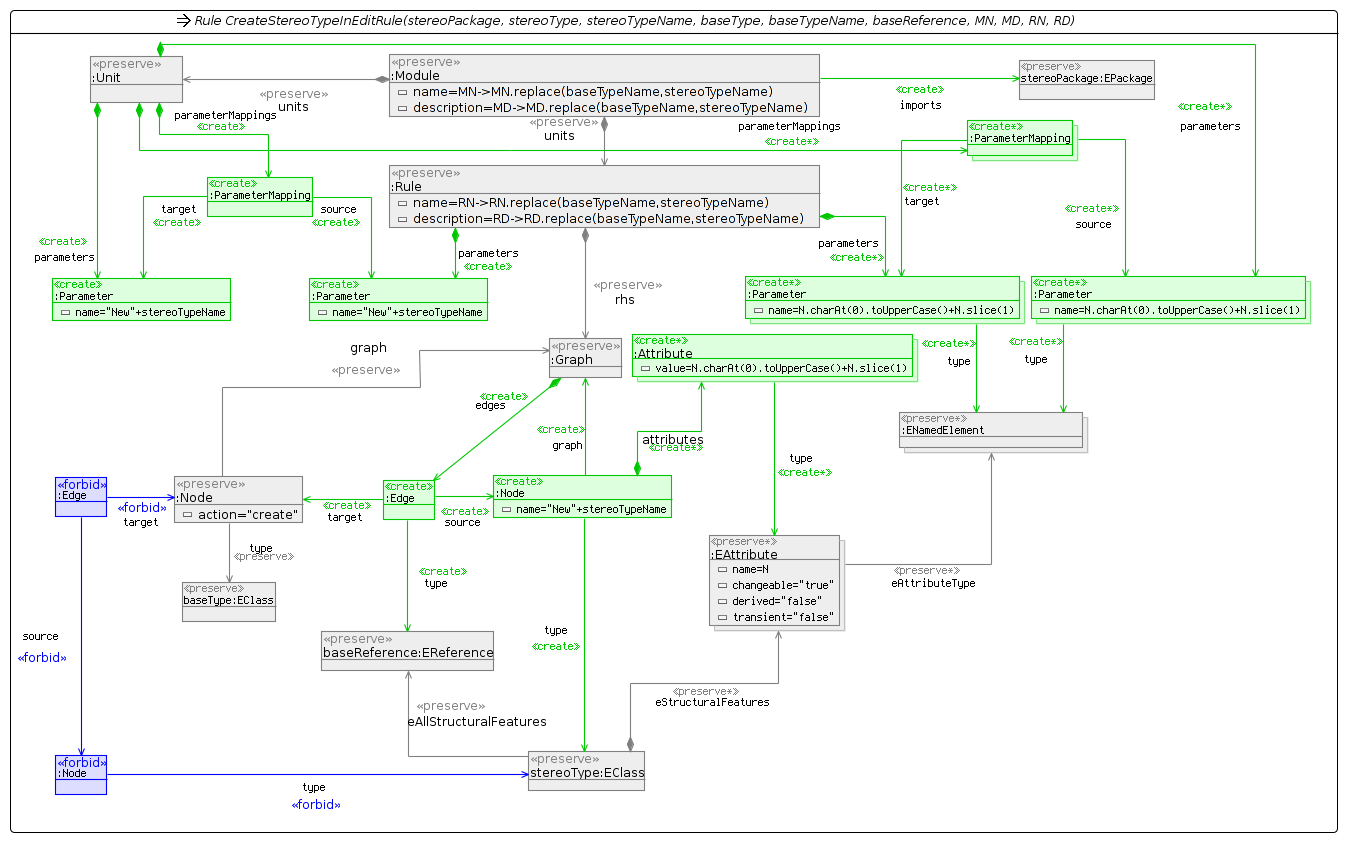
\includegraphics[scale=0.6, angle=90]{CREATE_STEREOTYPE_IN_EDITRULE}\\
\end{center}
\caption[]{\ac{HOT} for create nodes}
\label{hot_create}
\end{figure}
\newpage
\begin{figure}[h!]
\begin{center}
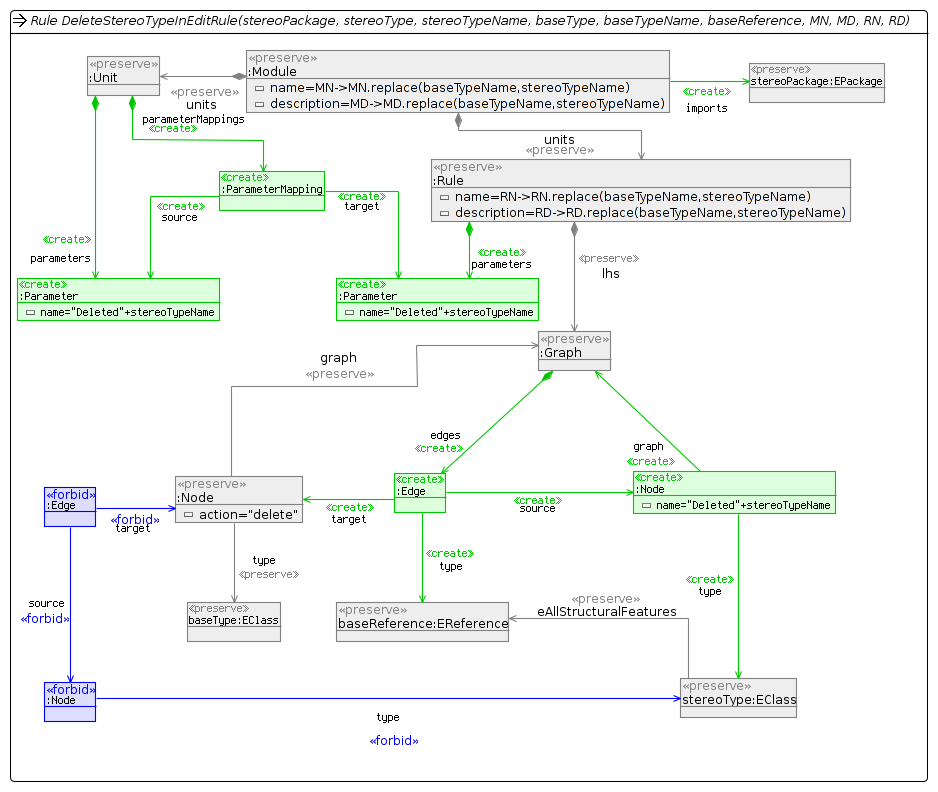
\includegraphics[scale=0.6, angle=270]{DELETE_STEREOTYPE_IN_EDITRULE}\\
\end{center}
\caption[]{\ac{HOT} for delete nodes}
\label{hot_delete}
\end{figure}
\newpage
\begin{figure}[h!]
\begin{center}
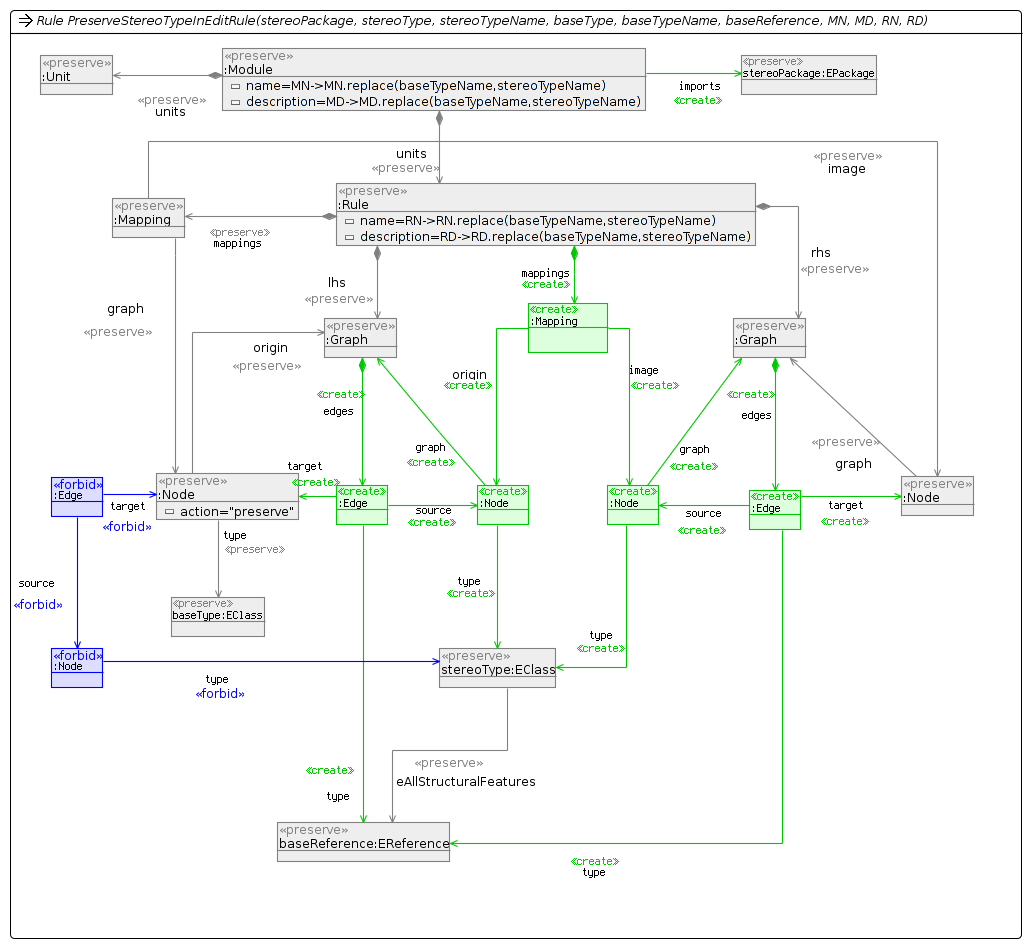
\includegraphics[scale=0.55, angle=90]{PRESERVE_STEREOTYPE_IN_EDITRULE}\\
\end{center}
\caption[]{\ac{HOT} for preserve nodes}
\label{hot_preserve}
\end{figure}
% \chapter{SiDiff UML configurations}\label{appendix:sidiffcfgs}
% \lstset{
%     language=XML,    
%     morekeywords={encoding, documentType,
%     normalizeWeights, condition, policy, name,class,threshold,weight,parameter},
%     captionpos=top, caption={SiDiff \ac{UML} similarity configuration},
%     label=sidiffcfg_similarity
%     }
% \lstinputlisting{attachments/org.sidiff.sysml.core.compareconfig.xml}
% \newpage
% \lstset{
%     language=XML,    
%     morekeywords={encoding, documentType,
%     normalizeWeights, condition, policy, name,class,threshold,weight,parameter},
%     captionpos=top, caption={SiDiff \ac{UML} matching Sequence},
%     label=sidiffcfg_similarity
%     }
% \lstinputlisting[firstline=99,lastline=130]{attachments/org.sidiff.sysml.core.matchingconfig.xml}
\chapter{\ac{SysML} Case Study Evolution}\label{appendix:sysml_casestudy}
This appendix describes the evolution of the \ac{SysML} case study used
throughout this Master's Thesis in a detailed manner. This evolution has been
created by the technical university of Munich and the corresponding
publication~\cite{aiscasestudy} is recommended.
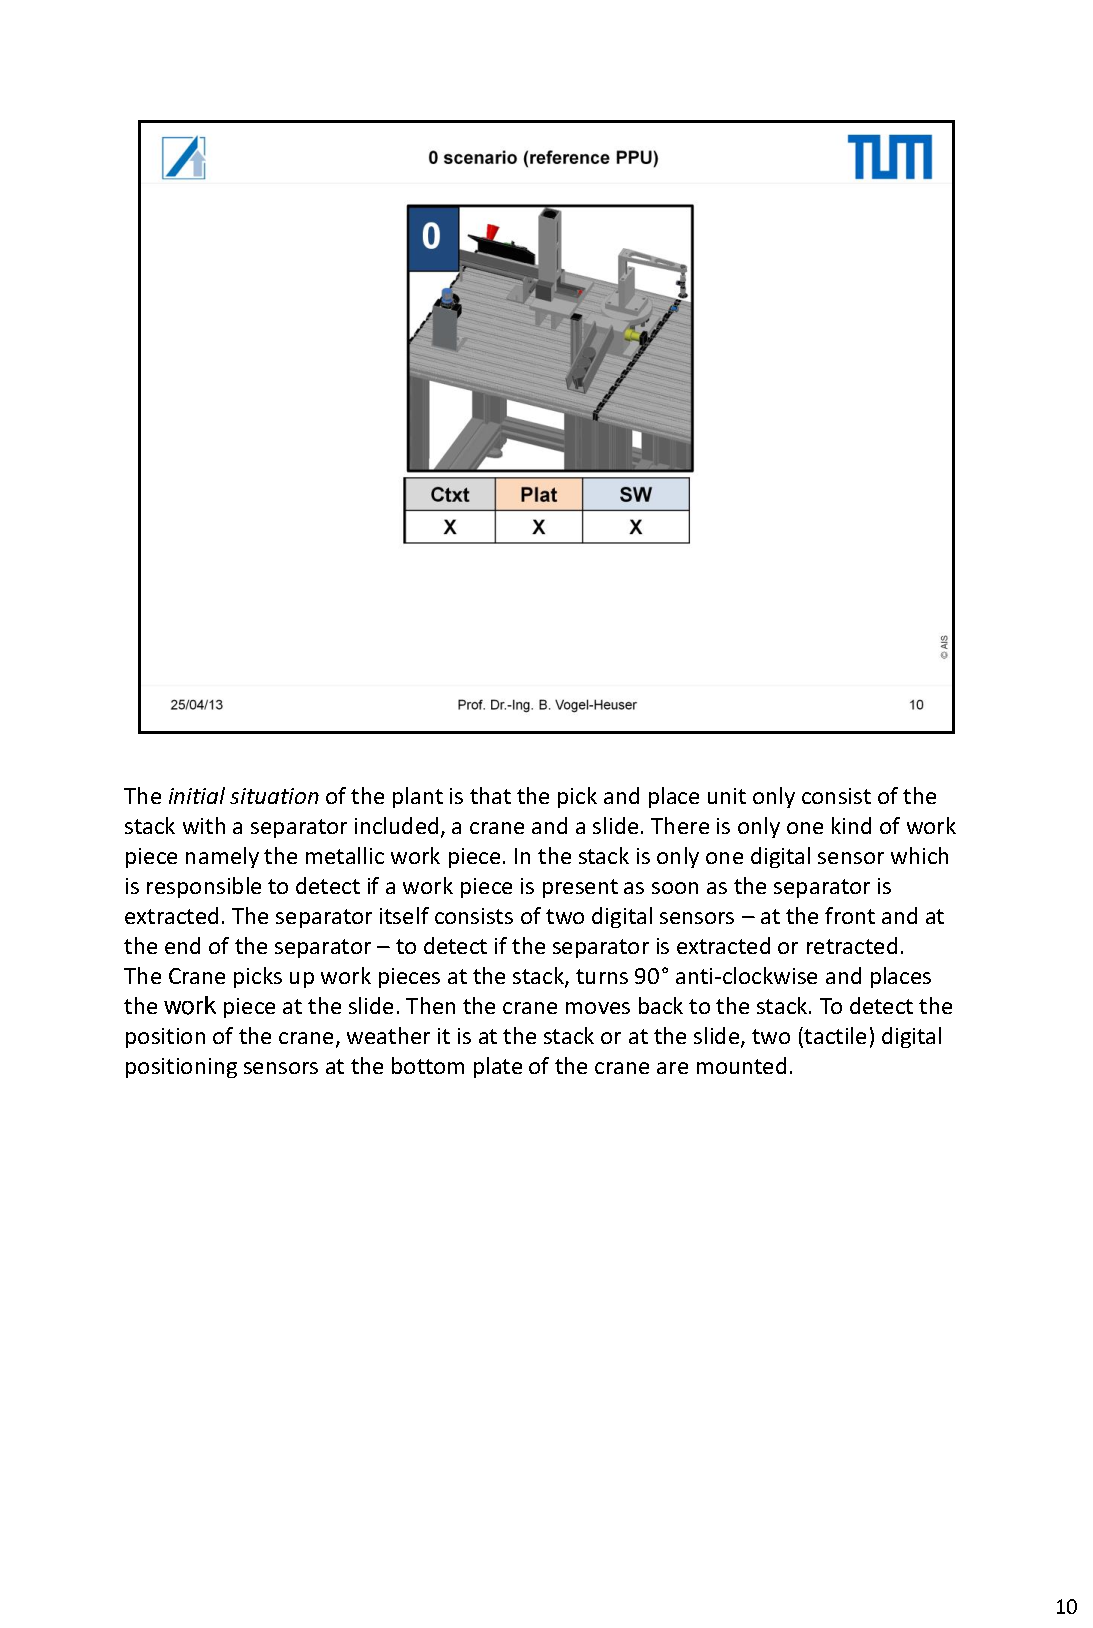
\includepdf[pages={-}]{attachments/Description_EvolutionScenarios.pdf}